% Based on OSDI template:
% https://www.usenix.org/sites/default/files/osdi_submit.tex_.txt

% comment out the following line to move from EuroSec template to OSDI template
\newcommand{\isworkshoppaper}{X}

\ifdefined\isworkshoppaper
\newcommand{\paperdocumentclass}{sig-alternate-05-2015}
\else
\newcommand{\paperdocumentclass}{article}
\fi

\documentclass[10pt,twocolumn]{\paperdocumentclass}

% template packages
\ifdefined\isworkshoppaper
\else
\usepackage{times}
\usepackage{fullpage}
\fi

% non-template packages
\usepackage[bookmarks=true,pagebackref=false,pdftex]{hyperref}
\usepackage{epsfig} % eps figures
\usepackage{graphicx}
\usepackage{epstopdf}
\usepackage{cite}
\usepackage{verbatim}
\usepackage{listings}
\usepackage{xcolor}

% variables
\newcommand{\projectname}[0]{METAlloc}

% comment out the following line to disable comments in text
%\newcommand{\commentsenabled}{X}
% comment commands
\ifdefined\commentsenabled
\newcommand{\EK}[1]{\textbf{\color[rgb]{0,1,0} EK: #1}}
\newcommand{\IH}[1]{\textbf{\color[rgb]{1,0,0} IH: #1}}
\newcommand{\CRI}[1]{\textbf{\color[rgb]{0,0,1} CRI: #1}}
\else
\newcommand{\EK}[1]{}
\newcommand{\IH}[1]{}
\newcommand{\CRI}[1]{}
\fi
\newcommand{\lipsum}[1]{{\color[rgb]{0.75,0.75,0.75} Lorem ipsum dolor sit amet, consectetur adipiscing elit, sed do eiusmod tempor incididunt ut labore et dolore magna aliqua. Ut enim ad minim veniam, quis nostrud exercitation ullamco laboris nisi ut aliquip ex ea commodo consequat. Duis aute irure dolor in reprehenderit in voluptate velit esse cillum dolore eu fugiat nulla pariatur. Excepteur sint occaecat cupidatat non proident, sunt in culpa qui officia deserunt mollit anim id est laborum.}}



\lstset{language=C++, 
    frame=lines, 
    backgroundcolor=\color{white},
    basicstyle=\scriptsize,
    %numbers=left,
    breaklines=true,
    tabsize=2,
    captionpos=b,
    commentstyle=\color{gray}\ttfamily,
    xleftmargin = 6pt,
}

\hypersetup{
unicode,
% no color links
colorlinks=true,
citecolor=black,
filecolor=black,
linkcolor=black,
urlcolor=black
} 

% hacks
\newenvironment{code}{\small\verbatim}{\endverbatim\normalsize}
\newcommand{\note}[1]{\noindent\textbf{\color{red}[#1]}}
\newcommand{\commentout}[1]{}

\begin{document}

\ifdefined\isworkshoppaper
\title{\projectname{}: Efficient and Comprehensive Metadata Management for Software Security Hardening}
\else
\title{\bf \projectname{}: title goes here} % TODO put title here
\fi

\ifdefined\isworkshoppaper
\author{
	Istvan Haller \\ Vrije Universiteit Amsterdam \\ \texttt{i.haller@student.vu.nl} \and 
	Erik van der Kouwe \\ Vrije Universiteit Amsterdam \\ \texttt{vdkouwe@cs.vu.nl} \and 
	Cristiano Giuffrida \\ Vrije Universiteit Amsterdam \\ \texttt{giuffrida@cs.vu.nl} \and 
	Herbert Bos \\ Vrije Universiteit Amsterdam \\ \texttt{herbertb@cs.vu.nl}}
\else
\author{Paper \# XXX} % TODO put paper number here, no author names as submission is double-blind
\fi

\date{}
\maketitle
\thispagestyle{empty}

\begin{abstract}

Many systems software security hardening solutions rely on the ability to look up
metadata for individual memory objects during the execution,
but state-of-the-art metadata management schemes incur significant lookup-time or allocation-time overheads and are unable to handle different memory objects (i.e., stack, heap, and global)
in a comprehensive and uniform manner.

We present \projectname{}, a new memory metadata management scheme which
addresses all the key limitations of existing solutions. Our design relies
on a compact memory shadowing scheme empowered by an alignment-based object allocation strategy. \projectname{}'s allocation strategy ensures that all the memory objects within a page share the same alignment class and each object is always allocated to use the largest alignment class possible. This strategy provides a fast alignment-based memory-to-metadata mapping, while minimizing metadata size and reducing memory fragmentation. We implemented and evaluated \projectname{} on Linux
and show that \projectname{} incurs just 1.2\% run-time performance overhead, paving the way for practical software security hardening in real-world deployment scenarios.
\looseness=-1
\end{abstract}

\section{Introduction}
%1) Problem, vulnerabilities and impact, 
Many system applications are written in unsafe languages like C/C++. These languages are mostly used to have explicit control over hardware interfaces for optimal performance. For example, pointers are used to have explicit control on memory management. However, incorrect use of explicit control can lead to security vulnerabilities. Pointers incorrect use may lead to memory corruption. Use of dangling pointer is one instance of incorrect behaviour. \\

%2)Use-After-Free vulnerability
% \textbf{Mention stats and impact of recently.}\\
Dangling pointer is a pointer that points to the freed object. Use of dangling pointers i.e. Use-after-Free or Double-Free affects application integrity, availability and confidentiality~\cite{CVEMitre}. Dangling pointer may write invalid data into newly allocated memory resulting into data corruption, thereby affecting integrity. Memory allocators consolidate two adjacent freed chunks into single big chunk. When Use-after-Free occurs after chunk consolidation, invalid data can be used as chunk information. This state results into free-list corruption that can lead to application crash, thereby affecting availability. Moreover, Use-after-Free before chunk consolidation is prone to arbitrary code execution, thereby affecting confidentiality. Segmentation fault due to Use-after-Free can leak memory addresses, thereby making Address Space Randomization (ASLR) protection weak ~\cite{serna2012info}. Also, Use-after-Free vulnerabilities are reported and exploited in widely used browsers~\cite{tutorial2010internet, IRCVE}. Most of the highly critical vulnerabilities can be exploited with low complexity. The impact includes unauthorized information disclosure/~modification or service disruption ~\cite{NVDNist}. \\

%3) mitigation techniques
%\textbf{Undangle, Cling and other.Add techquines that are used in the past to mitigate dangling pointers exploit.}
% WE should mention what is pointer-object relationship briefy. with common development practice is to set NULL.s 
Common defensive coding practice is to set dangling pointer to benign value \texttt{NULL}. Manually, this practice is not scalable in large code base when multiple pointer copies are present. Same technique can be used dynamically to track all pointers to the object and set pointer value to \texttt{NULL} when object is freed. State-of-the-art mitigation techniques like \dangnull{} ~\cite{lee2015dangnull}, \freesentry{}~\cite{younan2015freesentry} tracks pointer-object relationship dynamically (during run-time). Compiler infrastructure like CIL ~\cite{necula2002cil}, LLVM~\cite{lattner2004llvm} is used to insert run-time pointer tracking functions. \dangnull{} uses red-black tree data structure to store and retrieve metadata (i.e. pointer-object relationship). It provides thread-safety for data structure operations using mutexes. However, \dangnull{} incurs high average performance overhead of $80\%$. Also, it does not track stack and global pointers. \freesentry{} has an average performance overhead of $25\%$. This performance is reported using CIL for static instrumentation. Performance numbers with LLVM are higher than CIL~\cite{freesentrypppt}. \freesentry{} uses hash-table to store and retrieve metadata. However, thread-safety for data structure protection is missing in \freesentry{}. Thus, it can break multi-threaded (production) applications. Also, \freesentry{} has not evaluated throughput degradation of web-servers. Therefore, state-of-the-art mitigation techniques either incur high performance overhead or have limited applicability. \\% Should we write missing throughput numbers for webservers

%4) Brief about first design 
In dynamic analysis, pointer-object relationship is tracked. To store and retrieve relationship information, we need highly efficient and complete shadow memory management framework. It should have low lookup and memory overhead. \metalloc{} ~\cite{istvan2016metalloc} is an efficient metadata management scheme. We first evaluated effectiveness of metadata management framework, \metalloc{}. We implemented \freesentry{} scheme using \metalloc{}. We found that thread-safety (i.e. data structure protection) introduces huge performance overhead of $70\%$. Applications in production environment are highly multi-threaded. We have proposed simple and fast lock-less Use-after-Free detection scheme, called as \projectname{} to protect multi-threaded applications efficiently. \projectname{} maintains per-Thread and per-Object metadata, thereby it reduces thread synchronization. We implemented \projectname{} using \metalloc{}. \projectname{} has moderate run-time overhead of $43.9\%$ when only heap pointers are tracked. Moreover, it introduces only $4\%$ more overhead when all pointers are tracked (Stack, Heap and Global).

\input{metalloc}
\section{Applications}
\label{sec:applications}
\CRI{I suspect this section will have to go for EuroSec (and be condensed as a couple
of examples in the intro.)}

Efficient metadata tracking enables a wide range of valuable instrumentation
tools to be used with production systems where performance overhead is a
key characteristic. In the following we present a couple of key examples 
of such instrumentation.
% and their design relative to \projectname{}. 
This list is by no means exhaustive and we hope that readers
find other innovative uses of the framework. In this (short) paper, the applications  serve as motivation for our work and we will focus our evaluation on the framework itself.

\subsection{Write Integrity Protection}

Recent developments in attack techniques~\cite{carlini2015control,evans2015control,schuster2015counterfeit}
show the need to enforce additional data 
integrity within the program besides the classic control-flow integrity. 
Both Microsoft's WIT~\cite{akritidis2008preventing} and Oracle Application Data Integrity have looked into the 
topic of restricting the target addresses of memory writes using a coloring mechanism. 
In these schemes each memory location is associated with a given color and the instrumentation
alongside each memory write checks if the target location matches the color of
the pointer/instruction.
The major difference between the two schemes is the availability
of pointer color in the Oracle implementation stemming from a custom extension in
their latest CPU design. Microsoft on the other hand computes static colors for
the instruction based on points-to analysis.
In the case of both of these systems, the color for the memory location is tracked
using metadata shadowing with a fixed compression ratio.
Replacing these systems with \projectname{} can lead to substantial improvements  in  allocation performance.

In the case of both of these systems, the color for the memory location is tracked
using metadata shadowing with a fixed compression ratio. Thus integrating \projectname{}
into these systems is trivial, bringing with it all the advantages of variable compression ratio,
namely lower memory overhead and lower allocation overhead. However it does introduce
overhead when retrieving the metadata as the metadata information also needs to
be retrieved for the memory page corresponding to the pointer. In practice Write Integrity Protection
requires the most frequent metadata retrieval out of all the presented applications, showcasing the
worst case behaviour of \projectname{}.
\begin{comment}
To measure the effects of integrating \projectname{} into these systems, we
reimplemented the Microsoft scheme in a simplified manner. We use the DSA inter-procedural
points-to analysis~\cite{lattner2007making} from LLVM to identify connections between instructions
and memory locations. Since we only care about the performance characteristics of the metadata
tracking component, the accuracy of DSA relative to the points-to analysis presented in
the WIT paper is irrelevant. We also replicate the original metadata tracking from WIT by fixing the compression
ratio to the proposed values and by using a shadow memory located at a fixed address, allowing us to
perform a fair comparison across more recent benchmarks.
We also preserve the original design using a single byte of color as metadata. The detailed comparison of
the different metadata tracking solutions for write integrity protection can be found in
section~\ref{sec:evaluation}.
\end{comment}

\subsection{Bounds Checking}

Efficient bounds checking has been proposed in the past to counter
buffer overflow vulnerabilities, but none of the solutions ended up in production systems
due to the performance and memory overheads they bring. One particularly efficient example is
Baggy Bounds Checking~\cite{akritidis2009baggy} which offers a strong protection model with limited memory overhead,
based on fixed compression metadata. Its primary deficiency is the need to allocate objects in slots
with sizes in the powers of two, a requirement that is typically not enforced in generic heap allocators
due to the potential for high internal fragmentation.
The system can be rebuilt without the alignment requirements but that would require tracking
base pointer and size information for every object, which leads to performance and memory issues with
the fixed compression ratio (it is prohibitive to store 16 bytes of metadata for every 8 data bytes).
\projectname{} and its variable compression ratio can help to deal with the problematic large object allocations,
ensuring consistently low overhead across applications even when using multiple metadata bytes.

For this application the design requires a 16-byte metadata including both base pointer and size information.
Metadata retrieval is performed whenever a potentially dangerous pointer is read from memory and bounds check is applied to
pointer arithmetic with the same logic as defined in Baggy Bounds Checking. Again metadata retrieval is more expensive than with
the shadowing approach, however it occurs significantly less frequently. Most of the time pointer arithmetic suggests accesses to
multiple different offsets relative to the same base pointer, allowing the instrumentation to reuse the pointer metadata for multiple
bounds checks.
\begin{comment}
\EK{ISTM it's not really the same because the alignment in baggy bounds checking makes the check simpler compare to base pointer/size}
Comparison against the original Baggy Bounds Checking is difficult without having access to the buddy allocator
(outside of the scope of this paper), but we can still observe the efficiency of the proposed framework,
which does not have any of the compatibility issues posed by the buddy allocator. 
\end{comment}

An alternative implementation of bounds checking is Light-weight Bounds Checking~\cite{hasabnis2012light}. 
This system detects out-of-bounds accesses at the memory access time
instead of during the pointer arithmetic. The system injects guard zones between objects
and fills them with a random byte value to detect any access into these regions. 
A memory access is safe if it returns a different value, but real data might also
accidentally match the guard value. An additional check is performed in
the latter case to filter out false positives, but on average it is only performed
with probability 1 in 256. This check retrieves a metadata bit associated with
the address which specifies if it belongs to real data or one of the guard zones.
Light-weight Bounds Checking uses a fixed compression ratio shadowing
scheme of one metadata bit for every byte of data in the program.
However, metadata retrieval is avoided on the fast-path of this scheme
with little impact on performance. As a result replacing the existing
metadata tracking with \projectname{} only yields benefits to the system.
The existing system uses a hierarchical metadata storage system requiring
two memory accesses to retrieve the metadata bit. \projectname{} also performs two
memory accesses, but it involves more pointer arithmetic instructions.
It is safe to say that the fast-path behaviour will easily hide the small difference
in retrieval overhead. On the other hand the variable compression ratio of \projectname{} reduces allocation overhead,
which can be significant in many applications. As a result,  Light-weight Bounds Checking can also benefit from using \projectname{} for its metadata tracking.
%\EK{IMO having this paragraph in the paper means we should also implement Light-weight Bounds Checking to verify our claims}

\subsection{Type Confusion Detection}

Recently type confusion vulnerabilities received significant attention as an
alternative memory corruption mechanism which is not covered well by static analysis and run-time checkers. 
Type confusion happens when pointers are allowed to be cast into invalid types
without checking the run-time type information. It typically occurs in large software
projects with extensive class hierarchies. The ``static'' cast feature in C++ triggers compile-time
checks when object pointers are being up-casted to base classes
(as the object type specifies if it is an instance of the base class), but allows unchecked
down-cast to the original object types (no way to infer the specific derived class of the object at run time). 
The ``reinterpret'' cast is even more dangerous as it involves no compile-time checks
while changing the type of the object pointer. Under normal circumstances ``dynamic''
casting should be used while down-casting, however it introduces a significant overhead
and is therefore not allowed in many large software projects~\cite{lee2015type}.

%
CaVer~\cite{lee2015type} was designed as an efficient system to dynamically track type information
and to perform type validation at potentially vulnerable cast locations.
It uses a metadata tracking mechanism from within LLVM (presented in section~\ref{sec:related}) 
for heap objects, but reverts to red-black trees for stack and global allocations. As such,
it requires additional operations during metadata retrieval to identify the type of the pointer.
By using \projectname{}, CaVer gains access to uniform pointer handling and low overhead
irrelevant of the memory usage pattern. This is especially beneficial when considering the excessive
overhead reported in CaVer for Firefox, which was attributed to its use of stack variables.

The proposed improvement of the metadata retrieval also means that the
type verification using THTables becomes the key performance bottleneck.
We propose an alternative type tracking representation to solve this issue.
In the case of THTables, the system traverses a listing of potential base classes to
find a match with the target type. Existing virtual table protection mechanisms~\cite{tice2014enforcing}
however show that it more efficient to create type sets instead. 
We expand on this notion to define CastSets. The CastSet of a particular aggregate
type includes all other aggregate types in the system explicitly defined as pointer compatible
(primary base classes or sub-structures residing at pointer offset zero). The CastSet corresponding to a
pointer is the CastSet corresponding to the object being pointed to, if and only if the pointer
is the base pointer of the object. If the pointer is pointing to a non-zero offset within the object,
then the appropriate CastSet of the underlying nested structure needs to be
retrieved for analysis. For this purpose we designed the TypeArray object to
describe all potential CastSets corresponding
to the different offsets within a type. These also support array abstractions and multiple levels
of nestedness for size and performance considerations, but we will skip the details for brevity.
Figure~\ref{fig:typeexample} presents a simple example of CastSet and TypeArray interaction.

\begin{figure}[t]
\center
  \includegraphics[width=2.8in]{figs/typeexample.eps}
  \caption{
  Example of the interaction between CastSet and TypeArray. For both inheritance and composition,
  the CastSet includes Element as the new type contains a nested Element object at offset 0. The
  TypeArrays include the type itself at offset 0,
  while including other nested types at different offsets, such as the second Element member in the case of the
  Composited class.
  }
  \label{fig:typeexample}
  \vspace{-1em}
\end{figure}

CastSets and TypeArrays are constructed at compile time and stored in global memory, with
the latter pointing to the appropriate CastSets. Type confusion detection requires that
the instrumentation identifies the base pointer of the object as well as the NestedTypeArray corresponding
to the object. This allows to system to retrieve the appropriate CastSet and to identify if the cast target
is within the allowed set or not. This information can be tracked with a simple 8 byte metadata scheme.
The first metadata corresponding to the object includes a pointer to the NestedTypeArray itself, while subsequent
metadata elements store the relative offset (negative) required to reach the base pointer of the object.
Together with the alignment information retrieved as part of the metadata retrieval process, this gives the
instrumentation all the information it needs to perform type confusion detection. Storing different types of
information in the metadata field adds additional complexity (branch for negative values), but it allows
for smaller metadata sizes and thus allocation-time overhead. For this application the 
metadata retrieval frequency is significantly reduced (only required for static down-casts),
thus we expect that this design is preferable to ensure minimal overhead.

\subsection{Dangling Pointer Detection}

Use-after-free vulnerabilities represent the most prominent attack vectors in today's browser landscape~\cite{lee2015preventing}.
While a lot of effort is invested to detect these vulnerabilities via static analysis and software testing,
they typically manifest in highly specialized contexts, making them hard to detect and to fix preemptively.
As such, a couple of systems have been suggested recently to mitigate the underlying reason for the vulnerabilities,
dangling pointers~\cite{lee2015preventing,younan2015freesentry}. These systems rely on tracking heap allocations and
their connectivity at run time. When an object is freed, the systems identify whether there are any pointers
still pointing into the object being released. These pointers are then set to a benign value of NULL to mitigate
potential memory dereferences using them.

Systems for tracking dangling pointers share an underlying design based on three core
data structures. The first is the object map, which identifies heap objects based on any pointer
into the object itself (at any offset). This is equivalent to object metadata tracking.
DangNull~\cite{lee2015preventing} uses red-black trees to track heap allocations, but as discussed
in section~\ref{sec:introduction}, this scheme is susceptible to heavy and unpredictable overhead.
FreeSentry~\cite{younan2015freesentry} uses a label based system, which is equivalent to the fixed
compression ratio metadata shadowing. This scheme offers
fast fixed-time metadata retrieval, but incurs significant allocation-time and memory overhead. In contrast,
\projectname{} combines low allocation- and  lookup overhead with efficient memory usage.

The second data structure is a pointer map, which maps locations storing pointers with information about the
pointer itself. This is essentially location-specific metadata, thus a hash table is the most appropriate
data structure (as no range lookups are required) and both systems use it. The last data structure is the collection
of pointer to object mappings. This structure is used to accumulate information about all incoming/outgoing pointer
for a particular object.  Outgoing pointers are best tracked using a red-black tree as performed in DangNull to
allow efficient retrieval of the outgoing pointer residing at a particular offset in the object. FreeSentry on the
other hand tracks only incoming pointers which can be stored in a simple linked list instead. The disadvantage of
tracking only incoming pointers, is the difficulty of inferring if the source object of the incoming pointer is
still live in memory or not.

We propose a new dangling pointer tracking scheme inspired by FreeSentry, but using \projectname{} to track
object information. The proposed scheme tracks for each heap object the head of the
incoming pointer list as well as a unique identifier to help with object liveness. For each incoming pointer
we track the identifier of the source object, its base address, the address in memory where the pointer is stored
and the pointer value itself.
A hash table is used to map memory
locations with pointers stored within. Each pointer is represented by a link to the appropriate incoming pointer
element described previously. When a pointer is stored in memory, the old incoming pointer is destroyed and a new
one is created and prepended to the list of the target object. Then a link towards this element is stored in the appropriate
hash table location. When an object is freed, the system looks up the incoming pointer list checking if any of the entries
are still valid. An entry is valid if the specified source object still resides at the specified base pointer (based on the
unique identifier) and if the pointer location still contains the specified pointer value. For all valid entries the value stored
in the pointer location is reset to NULL to ensure no use-after-free vulnerabilities can exist. Figure~\ref{fig:metasentry}
showcases the data-structures described above.

\begin{figure}[t]
\center
  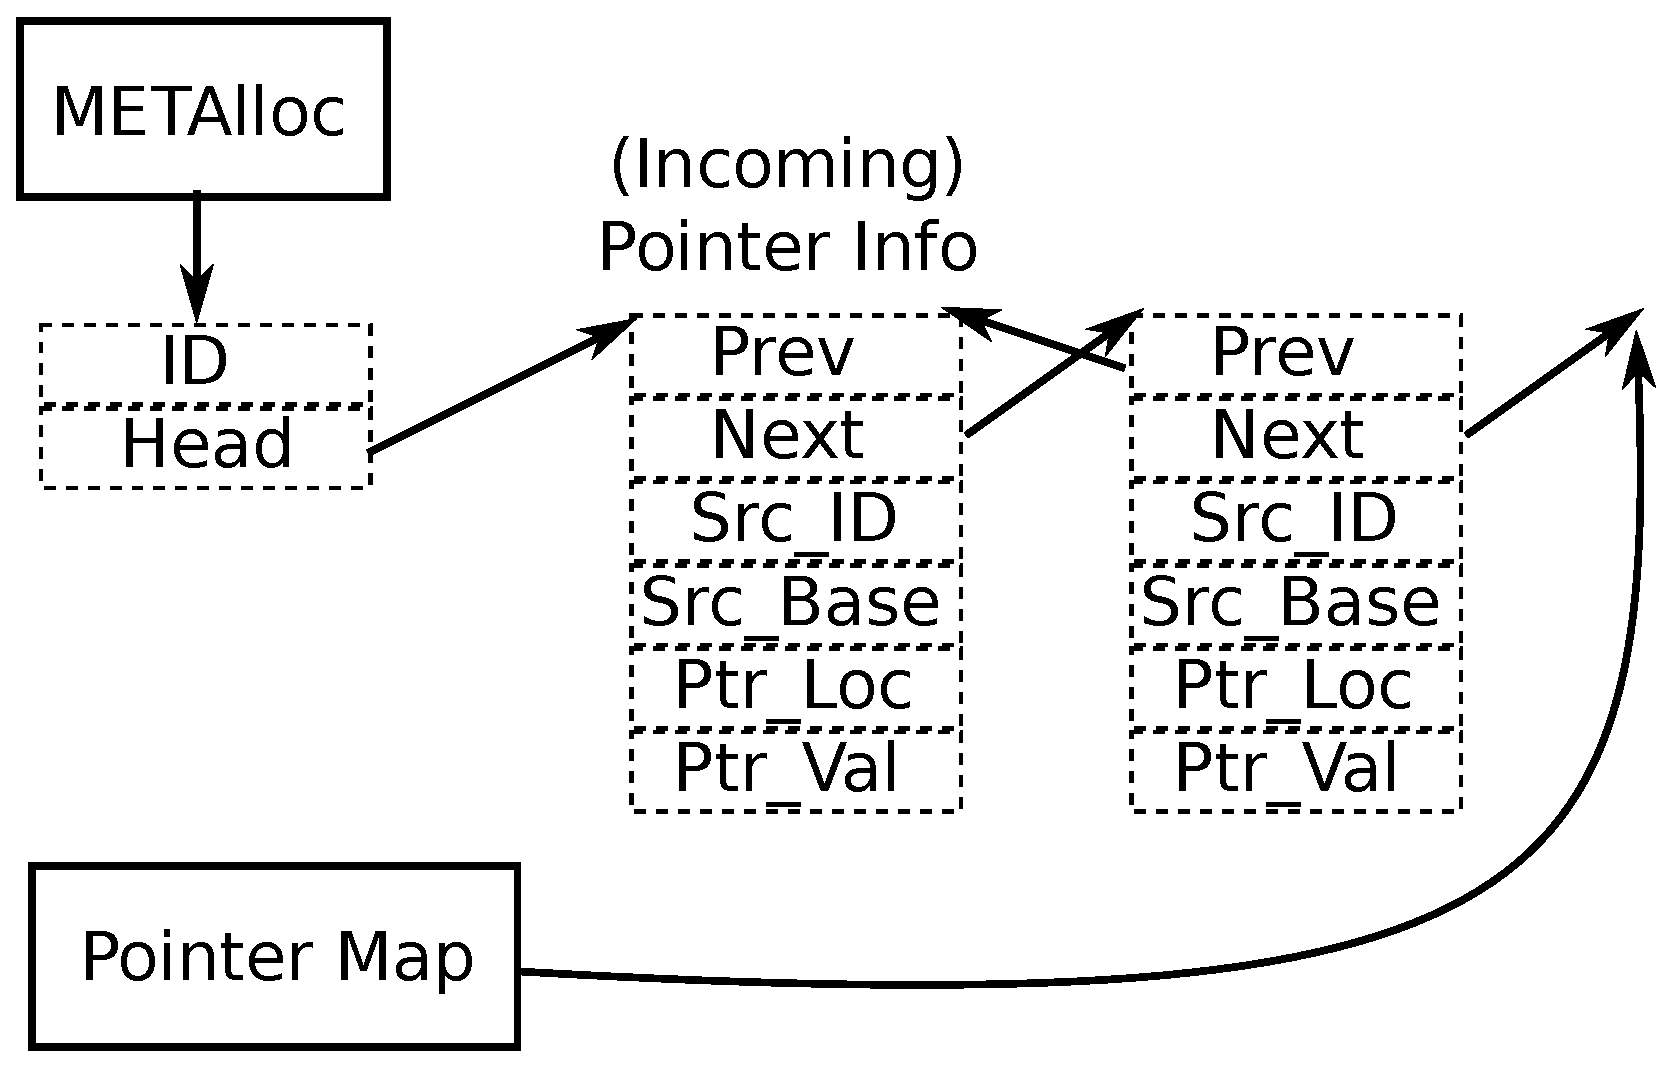
\includegraphics[width=2.8in]{figs/metasentry.eps}
  \caption{
  Data-structures used to implement dangling pointer detection using \projectname{}.
  \projectname{} allows the retreival of a unique object ID as well as a pointer to the head
  of a doubly linked list including information about incoming pointer information. The Pointer Map
  is used to retrieve the pointer infromation corresponding to a pointer stored in a given location.
  For each pointer we store information about the object containing it (ID and base address) as well
  as the location storing the pointer and the pointer value itself to allow nullification.
  }
  \label{fig:metasentry}
  \vspace{-1em}
\end{figure}

\section{Evaluation} \label{evaluation}
\begin{table}[t]
	\begin{tabular}{l*{4}{c}}
		\toprule
		\multirow{2}{*}{\bfseries Benchmarks} & \multicolumn{2}{c}{\bfseries \begin{tabular}{@{}l@{}} Normalized \\ with Baseline \end{tabular}} & \multicolumn{2}{c}{\bfseries \begin{tabular}{@{}l@{}} Normalized \\ with SafeStack \end{tabular}} \\%& \multirow{2}{*}{\bfseries \begin{tabular}{@{}l@{}} Number of tracking \\ functions inserted \end{tabular}} \\ % Great ;) hack to insert new line a cell
				
		\hhline{~----} & \begin{tabular}{@{}l@{}} Heap \\ Pointers \end{tabular} & \begin{tabular}{@{}l@{}} All \\ Pointers \end{tabular} & \begin{tabular}{@{}l@{}} Heap \\ Pointers \end{tabular} & \begin{tabular}{@{}l@{}} All \\ Pointers \end{tabular} \\ 
		\toprule
    		
    		\csvreader[head to column names]{Tables/spec_num.csv}{} % use head of csv as column names	
    		{\\\benchmark & \heapptrbaseline & \allptrbaseline & \heapptrsafestack & \allptrsafestack }%& \numinst} % specify coloumns here
    		\\
    		\bottomrule
	\end{tabular}
	
	\caption{SPEC2006 run-time overhead normalized with baseline and baseline-safestack. \projectname{} has $53\%$ run-time overhead compared to baseline numbers when only heap pointers are tracked, whereas $43\%$ compared to baseline-safestack. It has only $4\%$ more degradation when all pointers (Stack, Heap and Global) are tracked compared to when only heap pointers are tracked.}
	\label{table:spec2006}
	%\vspace{-1em}
\end{table}

\begin{figure}[t]
\center
  \includegraphics[width=3in]{plots/server_perf.eps}
  \caption{Web servers throughput degradation when compiled with \projectname{}. On an average throughput degradation is $12.8\%$ (compared to baseline-safestack). Negligible degradation in service latency.}
 \label{fig:server_perf}
  \vspace{-1em}
\end{figure} 

We evaluated \projectname{} in terms of performance overhead and effectiveness. We used CPU-intensive SPEC2006 performance benchmarks. For baseline configuration, we compiled benchmarks with clang/LLVM $3.8.0$. Moreover, we took numbers with one more baseline configuration (\emph{baseline-safestack}) with SafeStack option enabled. \metalloc{} handles stack objects similar to SafeStack. However, \projectname{} do not track stack objects. Therefore, we compare \projectname{} with baseline-safestack to remove run-time overhead introduced by stack objects handling. Both baseline configurations use unmodified \texttt{tcmalloc 4.2.6}~\cite{ghemawat2009tcmalloc} as a custom memory allocator. For \projectname{}, we compiled applications with our extra LLVM transformation pass to instrument the code. We linked \projectname{} run-time library statically with the application. We used custom inliner LLVM pass to inline most of the our run-time tracking functions. For all configurations, compiler optimization is set to \texttt{-O3}. We ran benchmarks on $64$-bit CentOS Linux with Intel Xeon CPU E5-2640 v3. We kept value of $\emph{N}\ =\ 3$, baselog size$\ =\ 8$ (number of pointers) with exponential log resize strategy.

\subsection{Performance Analysis} 
%\csvautotabular{Tables/spec_num.csv}

%%%%% Make comment for adding new line to the cell. Remove the hack

Table~\ref{table:spec2006} depicts run-time overhead of SPEC2006 benchmarks. Benchmark run-times are normalized with baseline and baseline-safestack. Stack pointers are short lived. That is, attacker has a very short time to exploit vulnerability. Use-after-Free exploits using stack dangling pointers are very rare. Performance overhead of tracking stack pointers is very high compared to its benefit. Therefore, we performed experiments for tracking all pointers (Stack, Heap and Global) and only heap pointers. Our static instrumentation has conservative approach. We end up instrumenting every pointer store instruction. We skip registration for invalid pointers and objects during run-time. This reduces large number of false negatives.  \projectname{} has average performance degradation (\textit{geomean}) of $53\%$ when only heap pointers are tracked. Moreover, it has only $4\%$ more (compared to only heap pointers tracking) overhead when all pointers are tracked. SafeStack has low performance degradation of $0.1\%$ ~\cite{kuznetsov2014code}. Compared to baseline-safestack, \projectname{} has average performance degradation of $44\%$ when only heap pointers are tracked. Similar to baseline, it has only $4\%$ more (compared to only heap pointers tracking) overhead when all pointers are tracked. \texttt{omnetpp} and \texttt{perlbench} have high performance degradation of $6x$ and $4x$ times, respectively. State-of-the-art Use-after-Free detection schemes have not included either \texttt{omnetpp} or \texttt{perlbench} overhead. Therefore, we cannot directly compare our average performance overhead with other recent schemes. When \texttt{omnetpp} is excluded, average performance overhead is $42\%$ (normalized with baseline) and $39\%$ (normalized with baseline-safestack) when all pointers are tracked. \\
% Include number of instruction instrumented %

% Server numbers and graph %/
Moreover, we evaluated \projectname{} on widely used web servers like \texttt{nginx}, \texttt{httpd} and \texttt{lighttpd}. We measured service latency (runtime) and throughput (Number of requests per sec) degradation. To measure service latency, we downloaded $2$GB file from server to client on localhost. We took average of $11$ runs. \projectname{} has shown negligible service latency degradation. To measure throughput, we used \texttt{ApacheBench}. We triggered $25000$ requests for static \texttt{index} page using $10$ concurrent requests. Figure~\ref{fig:server_perf} shows throughput degradation compared to baseline and baseline-safestack. \texttt{lighttpd} has low throughput degradation of $6.5\%$, whereas \texttt{nginx} and \texttt{httpd} has moderate degradation of $18.2\%$ and $17.7\%$, respectively. On an average (geomean), Web Servers have $12.8\%$ throughput degradation compared to baseline-safestack.     \\

% Run-time stats to explain more numbers
\begin{table*}[t]
\center
\begin{tabular}{l|*{6}{r}}
	\toprule
	\tablecell{Benchmarks} & \tablecell{Number of tracking \\ calls inserted} & \tablecell{Pointer \\ Registrations} & \tablecell{Duplicate \\ Pointers (\%)} & \tablecell{Objects \\ Allocated} & \tablecell{Objects \\ Free (\%)} & \tablecell{Log \\Overflows} \\
	\toprule
	\csvreader[head to column names]{Tables/spec_stats1.csv}{}
	{\\\benchmarks & \numinst & \ptrreg & \dupptr & \objalloc & \objfree & \logflow} \\% specify coloumns here
	\bottomrule
\end{tabular}
\caption{Run-time statistics for the SPEC2006 benchmarks}
\label{table:spec_stats}
\end{table*}

Furthermore, we collected run-time statistics to understand performance degradation. For this, we instrumented \projectname{} run-time library functions. Table~\ref{table:spec_stats}\ depict runtime statistics for SPEC2006 benchmarks compiled with \projectname{}. Column $2$ (Number of tracking calls inserted) represents a number of store instructions instrumented during static instrumentation phase. We have conservative static instrumentation pass. Therefore, we may end up instrumenting more than required. \texttt{gcc} and \texttt{xalancbmk} benchmark have almost $28K$ instrumented store instructions. Number of instrumented store instructions represent the number of pointer assignments found statically in the application. Column $3$ (Pointer Registrations) denotes a number of times run-time pointer tracking function is called. \texttt{gcc} and \texttt{xalancbmk} have more number of instrumented stores than \texttt{perlbench} and \texttt{omnetpp}. However, the number of run-time pointer tracking function calls are less. This is because same instrumented tracking function is called many times. It can happen when we instrument frequently executing application functions or loops. This information can be used to perform \projectname{} optimizations. Column $6$ represents number of allocated objects that are freed. Column $7$ shows the number of times log overflow occurred. Column $4$ shows percentage of  pointer registrations that are for \textit{Duplicate} pointers. For \texttt{lbm} benchmark, almost all pointer registrations are duplicates. For \texttt{sjeng} benchmark, pointer registrations are high with zero duplicates. It has only $5$ allocated objects and no log overflow. It can happen when pointer registration is called for a large number of invalid objects (Stack or Global) or pointers. \texttt{perlbench} and \texttt{omnetpp} have large number of object allocations and deallocations. Therefore, performance overhead for these benchmarks could be because of object allocations/deallocations. We initialize object metadata in allocation function and invalidate pointers in deallocation function. However, \texttt{dealII} and \texttt{xalancbmk} benchmark have more number of object allocations and deallocations than \texttt{perlbench}. Thus, performance overhead in \texttt{perlbench} seems to come from a large number pointer tracking function calls. As discussed earlier, these calls are from frequently executed application functions or loops. Therefore, advanced static instrumentation is required to avoid instrumentation for invalid store instructions. \\
%TODO Add for omnetpp

\textbf{Pointer Patterns.} 
We do not remove pointer registration from old objects metadata. Therefore, object log has large number of \emph{Duplicate} and \emph{Stale} pointers. We studied pointer pattern distribution (the number of \textit{Duplicate}, \textit{Unique} and \textit{Stale} pointers) in the log to fine-tune DangSan parameters.

\begin{figure*}[t]
\center
  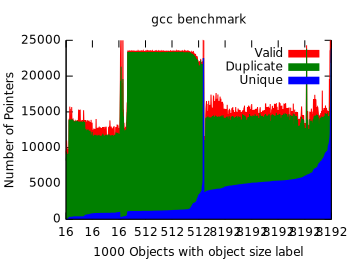
\includegraphics[width=2.8in,height=2.4in,keepaspectratio]{plots/gcc_pointerpattern.pdf}
  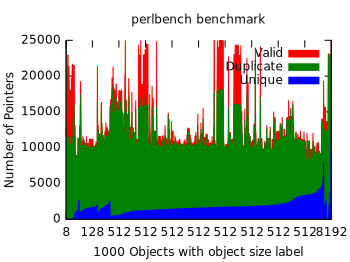
\includegraphics[width=2.8in,height=2.4in,keepaspectratio]{plots/perlbench_pointerpattern.pdf}
  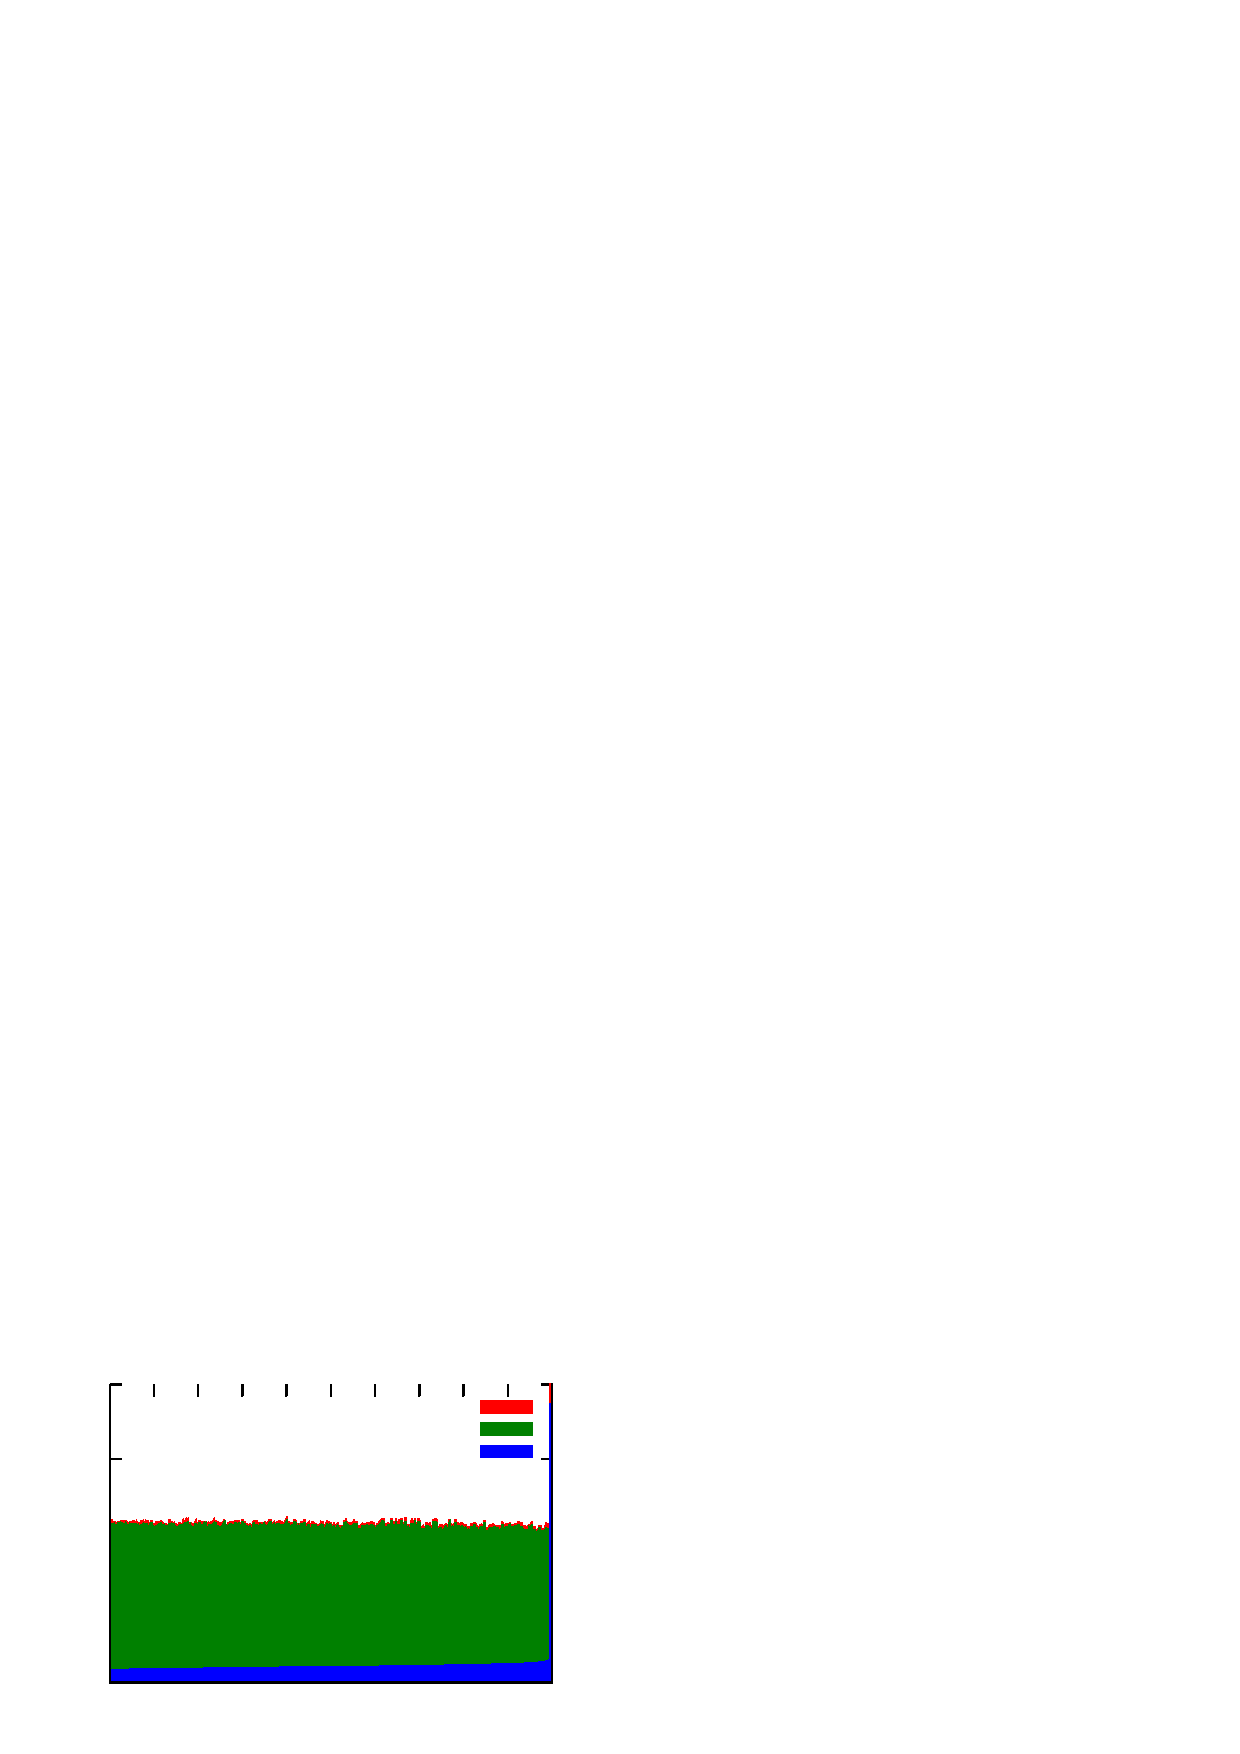
\includegraphics[width=2.8in,height=2.4in,keepaspectratio]{plots/astar_pointerpattern.pdf}
  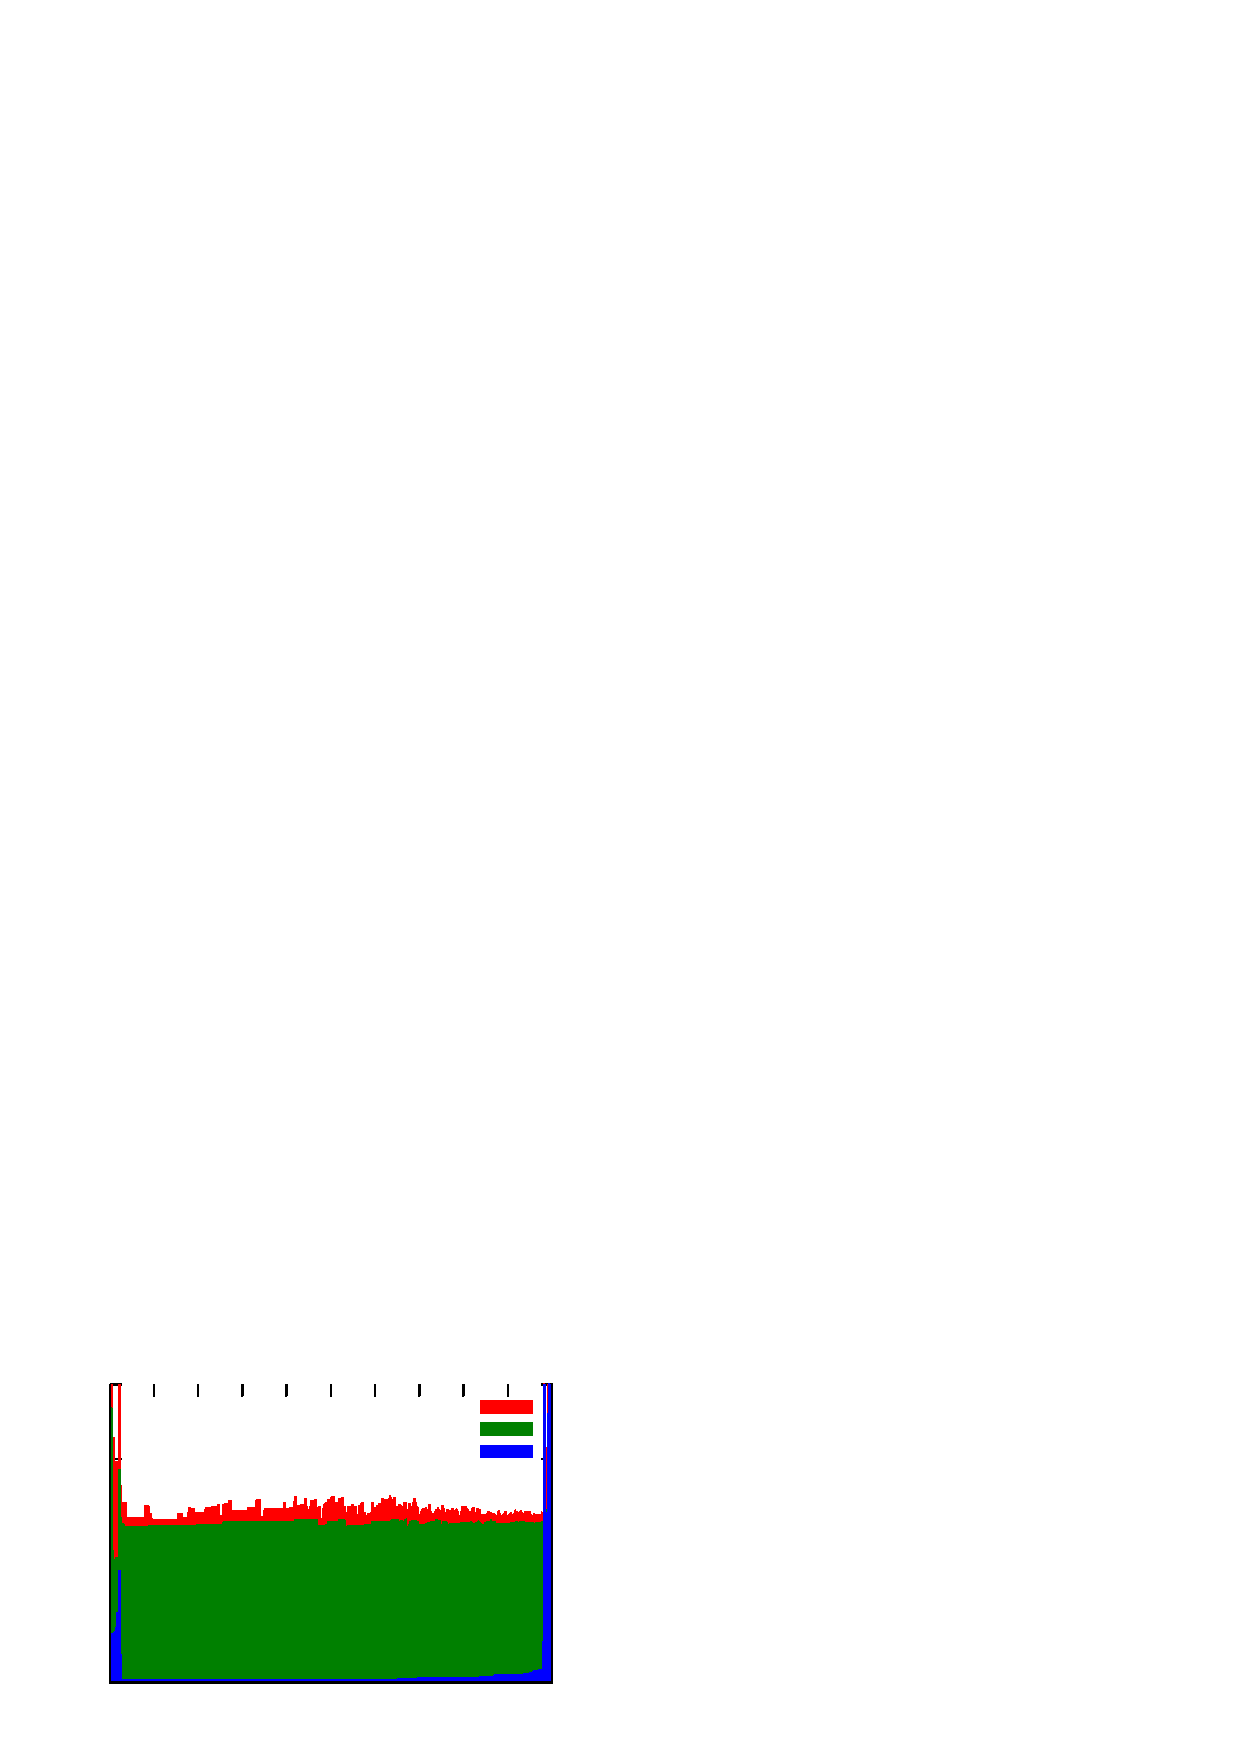
\includegraphics[width=2.8in,height=2.4in,keepaspectratio]{plots/xalancbmk_pointerpattern.pdf}
  
  \caption{Pointer registration pattern for the benchmarks that incur huge overhead. First $1000$ baselog overflow numbers are collected. N-Lookbehind value is $4$. Size of the baselog is kept very high to clearly visualize pattern difference.}
  \label{fig:pointerpattern}
  \vspace{-1em}
\end{figure*} 

Figure~\ref{fig:pointerpattern} shows pointer pattern distribution when a baselog overflow. We collected pointer pattern for first $1000$ objects that have overflown. The graph is plotted with increasing object size. Moreover, we collected statistics for benchmarks that incur huge overhead. Therefore, we chose two C benchmarks (\texttt{gcc} and \texttt{perlbench}) and two C++ benchmarks (\texttt{astar} and \texttt{xalancbmk}). We set baselog size to a very high value, $8K$ (number of pointers). Setting baselog size to a high value makes pattern clearly visible. We used \emph{N}-lookbehind value as $4$. In Figure~\ref{fig:pointerpattern}, red, green and blue area represents \textit{Valid}, \textit{Duplicate} and \textit{Unique} pointers, respectively. All four benchmarks have large number of \textit{Duplicate} pointers for any object size. Even after setting \emph{N}-Lookbehind value to $4$, \textit{Duplicate} pointers count is very high. Increasing value of \emph{N} may decrease \textit{Duplicate} pointers count but it has to trade-off with performance degradation. Furthermore, \emph{Unique} pointers count increases with object size for all the four benchmarks. Therefore, default baselog size should be proportional to the object size. However, it may introduce huge memory overhead. Next, the sum of \textit{Duplicate} and \textit{Unique} pointers represent the total number of pointers in the log. We store at max three pointers per log slot. Therefore, the total number of pointers per log can be at max $8K\ (log size) \times 3 = 24K$. For all the four benchmarks, on an average the total pointers count is above $11000$. In \texttt{gcc}, total pointers count reaches $23K$ for the object size $512$. That is, three times improvement in the memory utilization. Also, \textit{Valid} pointers count is very low for all the four benchmarks. Note, \textit{Valid} pointers count is inflated because pointers that are \textit{Duplicate} and \textit{Valid} are counted more than once. \textit{Valid} pointers count is very low even after counting \textit{Duplicate} and \textit{Valid} pointers more than once. Therefore, we need garbage collection of \textit{Stale} pointers to free the log space. \\

Furthermore, some pointers point to the same object but at different offset. These duplicate pointers may escape \emph{N}-Lookbehind strategy. We introduced one more strategy to remove these duplicate pointers. We compare old pointer value to the new object address range. When pointer points to the same object, we skip pointer registration. This \textit{Duplicate} pointers removal technique not only helps to remove \textit{Duplicate} pointers within a thread but also across threads. This technique removed $20\%\ to\ 25\%$ \emph{Duplicate} pointers for SPEC2006 benchmarks. For this technique, we need old pointer value in run-time tracking function. We slightly changed our static instrumentation pass. We insert run-time tracking function before store instruction instead of after store instruction. In run-time tracking function, we read old pointer value and check whether it still points to the same object. For fast check, we store object bound information in the object metadata. We store lowermost $32$-bits of object root address and object size together in the $64$-bit object metadata field. Therefore, \metalloc{} stores and retrieves $16$ bytes metadata, $8$ bytes for a pointer to a per-Thread log list and $8$ bytes for object information. \\

\subsection{Correctness}
We evaluated \projectname{} correctness on publicly available exploits. We chose following Use-after-Free (Double free) vulnerabilities. \\

\textbf{CVE-2010-­2939}~\cite{OpenSSLCVE}: This is a double free vulnerability in OpenSSL client version OpenSSL1.0.0a and function \texttt{ssl3\_get\_key\_exchange}. It is a highly critical vulnerability that results into denial of service or possible arbitrary code execution. We used exploit with the baseline configuration. It resulted into memory corruption error messages. Furthermore, we compiled OpenSSL1.0.0a with \projectname{}. We tried to exploit the compiled OpenSSL client. However, our system prevented double free. It aborted OpenSSL client due to invalid memory access.
\begin{verbatim}
src/tcmalloc.cc:290] Attempt to free invalid 
pointer 0x80000000022ba510 
./runclient: line 9: 20200 Aborted 
\end{verbatim} 
Above message indicates that our system had invalidated pointer by setting uppermost bit to $1$ when the object was freed first time.
 
\subsection{Memory Overhead}  
% Run-time stats to explain more numbers
\begin{table}[t]
\center
\begin{tabular}{l|*{3}{r}}
	\toprule
	\tablecell{Benchmarks} & \tablecell{Baseline \\RSS} & \tablecell{DangSan \\RSS} & \tablecell{Memory \\Overhead(MB)} \\
	\toprule
	\csvreader[head to column names]{Tables/spec_memory.csv}{}
	{\\\benchmarks & \baselinerss & \dangrss & \extramemory} \\% specify coloumns here
	\bottomrule
\end{tabular}
\caption{Memory overhead for the SPEC2006 benchmarks (MB)}
\label{table:spec_memory}
\end{table}

Table~\ref{table:spec_memory}\ shows memory overhead on SPEC2006 benchmarks introduced by \projectname{}. \texttt{perlbench}, \texttt{omnetpp}, \texttt{xalancbmk} and \texttt{astar} benchmarks have huge memory overhead in gigabytes. Memory overhead also comes from the metadata management scheme, \metalloc{}. \metalloc{} stores and retrieves $16$ bytes metadata for each object. It maintains metadata for all objects (including Stack and Global). We do not track Stack and Global objects. Thus, maintaining $16$ bytes metadata for Stack and Global object can inflate memory overhead numbers. Some defences may not require stack or global metadata management. One of the improvement required in \metalloc{} is to have selective metadata management. We believe that ~\metalloc{} will be used for other defences along with \projectname{}. Another reason for the memory overhead is, we increase one byte for every object allocation to solve \textbf{off-by-one} byte application compatibility issue. However, \texttt{tcmalloc} allocates object with powers of $2$ size. This tremendously increases memory overhead. One improvement to reduce memory overhead is to select additive increase log resize strategy. Table~\ref{table:spec_memory} also represents that increase in memory requirement increases performance overhead. This is directly proportional to the number of pointer propagations and object allocations. 
\section{Related work}
\label{sec:related}

Besides the different memory shadowing~\cite{akritidis2008preventing,akritidis2009baggy,younan2015freesentry}
and tree-based approaches~\cite{haller2013mempick,lee2015preventing} already discussed within this paper (in Sections~\ref{sec:introduction}
 and~\ref{sec:applications}) there is one system aiming
to solve the metadata tracking problem in a similar manner using a variable compression ratio. The
custom memory allocator implemented within the Sanitizer library of LLVM offers a metadata retrieval system,
which shares characteristics with \projectname{}. The system has been used within CaVer~\cite{lee2015type}
to track type information for heap objects, but is not described in other contexts.

This memory allocator reserves a specific part of the address-space
,as a Region, for each size category defined within the system. Regions are then split into slots of equal
size, with each slot containing a single object. This allows the allocator to associate each slot/object
with a singular piece of metadata, accessed by identifying the slot index corresponding to any pointer.
The Region is also easily identified from the pointer, since the organization of the address-space into
Regions happens at compile-time. This systems shares similarities with \projectname{}, with the primary difference being
the granularity of the memory blobs associated to a certain allocation size. \projectname{} only requires
memory pages to be uniform, which is already assured by the general purpose allocator \emph{tcmalloc}. This custom allocator
on the other hand restricts allocations within a certain Region, whose addresses are predefined at compile-time.
The result is a significant reduction of the potential for address-space randomization, with the address bits
of each Region being predictable by the attackers. Furthermore, the current implementation
also enforces a highly predictable allocation pattern within the Region itself with no ability to release
memory back to the system. The effort to add these highly desirable features to the current design is
unclear at this point. These concerns are of course irrelevant when using the allocator within the desired
context of software testing, but they are key characteristics for a general purpose production allocator.

While the design works efficiently for heap objects, Lee et al.~\cite{lee2015type} argue
that it is not directly applicable to stack and global memory. Their solution to the problem involves
integrating a tree-based metadata tracking for these memory types.
As far as we are aware, \projectname{} is the first design to combine uniformity across memory types with all the advantages
brought forward by variable compression ratio metadata tracking.

\section{Conclusion} \label{conclusion}
In this paper, we presented \projectname{}, a fast and efficient lock-less system to detect Use-after-Free exploits in multi-threaded applications. Thread-safety in multi-threaded program incurs prohibitively high run-time overhead. Our design (inspired from Log-structured file system) maintains per-Thread per-Object metadata that eliminates contention between threads. \projectname{} has moderate run-time overhead on CPU intensive benchmarks when all pointers (Heap, Stack and Global) are tracked. It has low throughput degradation for widely used WebServers. Our complete and efficient \projectname{} system can be used for large production applications.

%\projectname{} efficiently detects Use-after-Free exploit in Mul      


\bibliographystyle{abbrv}
\bibliography{refs}

\end{document}
